\section{Addressing the Identified Challenges}
All the challenges described in section \ref{sec:as-is-issues} have been analyzed, addressed, and resolved through a series of targeted interventions. 
These interventions concerned various aspects of the system, from restructuring the software architecture and revising data management processes to implementing new technologies and development practices. The solutions adopted for each of the identified challenges are detailed below.

\subsection{Architectural and Technological Challenges}
The adoption of an approach based on containerization (with Docker) and orchestration (with Kubernetes, often abbreviated as K8s) forms the foundation for overcoming the current architectural and technological limitations of the SRP system. This transition not only directly addresses issues of modularity, isolation, and dependency management but also paves the way for a more modern and scalable architecture, such as microservices or micro-frontends. Specifically, it aims to solve the problems of fragmentation, dependency complexity, and maintenance difficulties inherited from the previous monolithic architecture and the agent installed at the customer's site.

\subsubsection{Containerization with Docker}
Docker is a containerization platform that allows developers to package applications and all their dependencies (libraries, configurations, environments) into a single, standardized unit called a container. As illustrated in figure \ref{fig:docker-containers}, these containers are isolated from each other but share the host operating system's kernel, making them extremely lightweight and portable.

\begin{figure}[ht]
    \centering
    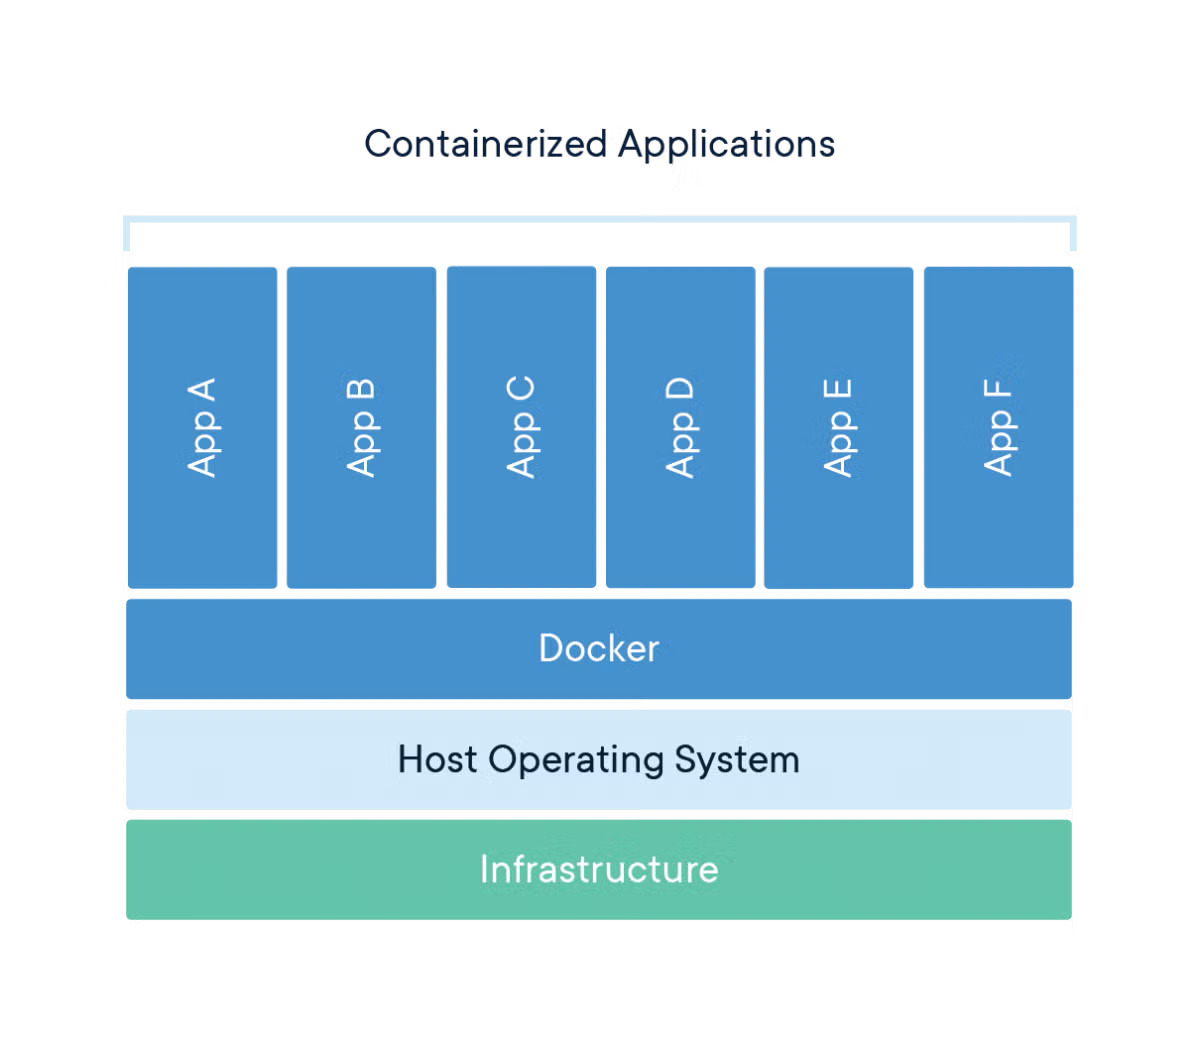
\includegraphics[width=0.7\textwidth]{images/architectural-redesign/docker containers.jpg}
    \caption{Docker Container Architecture (source: \cite{docker_doc})}
    \label{fig:docker-containers}
\end{figure}

The use of Docker resolves the "works on my machine but not in production" problem (known as "dependency hell") \cite{docker_swe} and provides a solid foundation for component decoupling. Each component (frontend, backend, support services) will be enclosed in a \textit{Docker container}, and ensures that the execution environment (including libraries, configurations, and dependencies) is identical across development, testing, and production \cite{docker_swe}. 
This eliminates errors caused by environmental discrepancies.

Once created, the container can be run anywhere Docker is present (in our case, container orchestration is managed by Kubernetes, which will be discussed in the next subsection), simplifying the deployment process. 
The system thus becomes extremely more portable, moving away from the strict dependence on specific operating systems and hardware configurations like, in this case, Windows Server and Microsoft SQL Server.

\subsubsection{Orchestration with Kubernetes}
Kubernetes (K8s) is an open-source system for automated container orchestration, originally developed by Google. Its purpose is to manage entire fleets of Docker containers in a \textit{cluster}, ensuring that applications are always available, scalable, and resilient \cite{kubernetes}.

If Docker provides the mechanism for creating and distributing containers, Kubernetes is its natural complement, handling their large-scale management (\textit{orchestration}), transforming the infrastructure from a set of single machines into a centrally managed cluster \cite{kubernetes}.

K8s allows components to scale horizontally based on the workload (via the Horizontal Pod Autoscaler). When demand increases, K8s automatically launches new instances of services (e.g., more pods for the REST backend) and removes them when the load decreases. This is crucial for managing traffic peaks \cite{kube_book}. 

In parallel, it constantly monitors the status of the containers. If a component fails, K8s automatically restarts it or schedules a new one on a healthy node in the cluster, ensuring high availability and resolving the single-point-of-failure problem introduced by the current dependence on single servers and the agent \cite{kube_book}. 

Kubernetes also supports advanced deployment strategies (e.g., Rolling Updates), allowing code updates without service interruptions (zero-downtime deployment) \cite{kube_book}. In case of issues, rolling back to the previous version is fast and automated. This mitigates the risk associated with system changes.

Finally, K8s also offers native mechanisms to manage environment variables and sensitive data (such as database credentials or external service authentication tokens) separately from the container code \cite{kube_book}. This centralizes management and increases security, eliminating the numerous hard-coded configurations present in the old system and making the containers more generic.

The adoption of Docker and Kubernetes therefore creates the ideal environment for the subsequent decomposition of the frontend monolith and the re-engineering of the various backend components, topics that will be covered in detail in the following sections.

\subsubsection{Monolithinc Frontend Component}

\subsubsection{Overly Generic Backend REST Services}

\subsubsection{Dependency on the SRP Agent}



\subsection{Code and Data Management Issues}

\subsubsection{Unversioned and Undebuggable Stored Procedures}

\subsubsection{Inaccessible and Unversioned SSIS Jobs}



\subsection{Database Schema and Data Integrity Issues}

\subsubsection{Lack of Data Integrity and Consistency}

\subsubsection{Data Redundancy}

\subsubsection{Unclear and Inconsistent Naming Conventions}



\subsection{Maintenance and Operational Challenges}
